\documentclass[12pt]{article}
\usepackage[a4paper, total={7.5in, 11in}]{geometry}
\usepackage{graphicx, subfig, wrapfig, fancyhdr, lastpage, multicol ,color,arydshln,makecell, mhchem}
\usepackage[mathscr]{euscript}
\usepackage{tabularray}

\newcommand\headerMe[2]{\noindent{}#1\hfill#2}

\setlength{\columnseprule}{1pt}
\def\columnseprulecolor{\color{blue}}


\pagestyle{fancy}
\fancyhf{}

\cfoot{ \vspace{-0.8cm}\em{Page \thepage \hspace{1pt} / \pageref{LastPage}}}
\begin{document}

\headerMe{Royaume du Maroc}{année scolaire \emph{2022-2023}}\\
\headerMe{Ministère de l'Éducation nationale, }{  Professeur :\emph{Zakaria Haouzan}}\\
\headerMe{du Préscolaire et des Sports}{Établissement : \emph{Lycée SKHOR qualifiant}}\\
\vspace{-1cm}
\begin{center}
Devoir Surveillé  N°1 \\
    2ème année baccalauréat Sciences physiques\\
Semestre 2 - Durée 2h00
\\
    \vspace{.2cm}
\hrulefill
\Large{Chimie 7pts - 42min}
\hrulefill\\

    %\emph{Les deux parties sont indépendantes}
\end{center}
%end Headerss------------------------
%__________________Chimie ______________________-
%%%%%%%+_+_+_+_+_+_+_+_+_Partie1
%\vspace{-1cm}
 \section*{Etude d’une solution aqueuse d’ammoniac \dotfill(7 pts) }
\begin{wrapfigure}[6]{r}{0.4\textwidth}
\vspace{-1.2cm}
\begin{center}
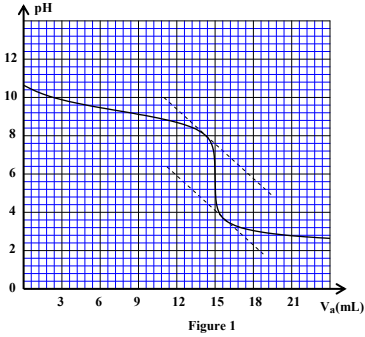
\includegraphics[width=0.4\textwidth]{./chimie00.png}
\end{center}
\end{wrapfigure}
\textit{L'ammoniac NH3 est un gaz qui, dissous dans l’eau, donne une solution basique d'ammoniac. Des
solutions commerciales d'ammoniac sont utilisées, après dilution, comme produits de nettoyage.}
Cette partie de l’exercice se propose d’étudier une solution aqueuse d’ammoniac.
On prépare une solution aqueuse $S_b$, de volume V, en diluant 100 fois une solution commerciale
d’ammoniac $S_0$ de concentration $C_0$.

\textbf{Données : } 
\begin{itemize}
	\item Toutes les mesures sont effectuées à 25°C.
	\item Le produit ionique de l’eau : $K_e = 10^{-14}$.
\end{itemize}

\textbf{1. Dosage de la solution Sb:}

On réalise un dosage pH-métrique d’un
volume $V_b = 15 mL$ de la solution $S_b$ de

concentration Cb par une solution aqueuse
Sa d'acide chlorhydrique $({H_3O^+}_{(eq)} + Cl^-_{(eq)})$ 
de concentration $C_a = 10^{-2} mol.L^{-1}$.

La courbe de la (figure 1) représente les
variations du pH du mélange en fonction
du volume $V_a$ versé de la solution $S_a$: $pH = f(V_a)$

\begin{tabular}{c|l}
	0,5  & \makecell[l]{ \textbf{1.1. }Ecrire l’équation de la réaction de dosage. }\\
	0,25  & \makecell[l]{ \textbf{2.2. }Ecrire, à l'équivalence, la relation entre $C_b$, $C_a$, $V_b$ et $V_{aE}$ le volume versé de la solution \\$S_a$ à
l'équivalence. }\\
	1,5  & \makecell[l]{ \textbf{3.3. }Montrer que la concentration de la solution $S_b$ est: $C_b = 10^{-2}mol/L$. En déduire $C_0$. }\\
	0,5 & \makecell[l]{ \textbf{4.4. }Choisir, parmi les indicateurs colorés suivants, l’indicateur adéquat pour réaliser ce dosage.
\\Justifier votre réponse.}\\ 
	\end{tabular}

	\begin{center}
\begin{tabular}{|c|c|c|c|}
	\textbf{Indicateur coloré} & hélianthine & rouge de méthyle & phénolphtaléine \\
	\textbf{Zone de virage} & 3,1 - 4,4 & 4,2 - 6,2 & 8,2 - 10 \\  
\end{tabular}
\end{center}


\textbf{2. Etude de la solution $S_b$:}

La mesure du pH de la solution aqueuse Sb donne: pH = 10,6.

\begin{tabular}{c|l}
	0,25  & \makecell[l]{ \textbf{2.1. }Ecrire l’équation de la réaction de l’ammoniac avec l’eau.}\\
	1  & \makecell[l]{ \textbf{2.2. }Calculer la concentration molaire effective des ions hydroxyde $HO^-$ dans la solution $S_b$.}\\
	1  & \makecell[l]{ \textbf{2.3 }Calculer le taux d’avancement final $\tau$ de cette réaction. }\\
	1  & \makecell[l]{ \textbf{2.4 }Vérifier que le quotient de la réaction à l’équilibre est: $Q_{r,eq} = 1,65.10^{-5}$ }\\
	1  & \makecell[l]{ \textbf{2.5 }En déduire la valeur du $pK_A$ du couple $NH^+_4/NH_3$. }\\
	\end{tabular}
%\hrulefill
%\Large{Physique 13pts/78min}
%\hrulefill\\
%	\vspace{3cm}
\begin{center}
    %\vspace{.60cm}
\hrulefill
\Large{Physique 13pts - 78min}
\hrulefill\\
    \emph{Les  parties sont indépendantes}
\end{center}

\section*{Partie 1 : Réponse d’un dipôle RC à un échelon de tension\dotfill(2pts)}
\begin{wrapfigure}[9]{r}{0.3\textwidth}
\vspace{-1.2cm}
\begin{center}
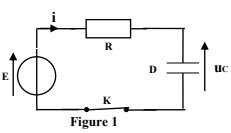
\includegraphics[width=0.3\textwidth]{./Rc00.png}
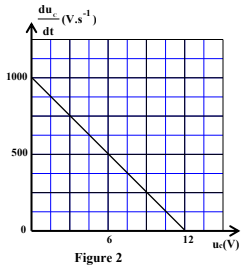
\includegraphics[width=0.3\textwidth]{./rc01.png}
\end{center}
\end{wrapfigure}


On réalise le montage, représenté sur le schéma de
la figure 1, constitué des éléments suivants :
\begin{itemize}
	\item Un générateur idéal de tension de force électromotrice E
	\item Un condensateur D de capacité C initialement déchargé
	\item Un conducteur ohmique de résistance $R = 10^3\Omega$.
	\item Un interrupteur K.

\end{itemize}
On ferme l’interrupteur à un instant choisi comme origine des
dates t = 0. Un système d’acquisition informatisé permet de
tracer la courbe de la figure 2, représentant les variations de $\frac{du_c}{dt}$
en fonction de $u_c$. 
$u_c$ étant la tension à un instant t.

\begin{tabular}{c|l}
	1 & \makecell[l]{ \textbf{1.1. }Montrer que l’équation différentielle vérifiée par la tension $u_c(t)$ \\s’écrit sous la forme :$\frac{du_c}{dt} = -\frac{1}{RC}.u_c + \frac{E}{RC}$ } \\

	1 & \makecell[l]{\textbf{1.2. }En exploitant la figure 2 , montrer que la capacité du
	\\condensateur est : $C = 12\mu F$ }\\
\end{tabular}

\section*{Partie 2 : Réponse d’un dipôle RL à un échelon de tension \dotfill(3pts) }
On réalise le montage schématisé sur la figure1.
Ce montage comporte :

\begin{center}
  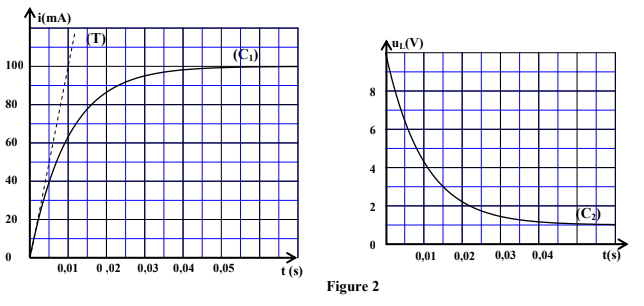
\includegraphics[width=1\textwidth]{./Rl00.png}
\end{center}

\begin{itemize}
	\item Une bobine d’inductance L et de résistance r.
	\item un conducteur ohmique de résistance $R = 90 \Omega$
	\item un générateur de force électromotrice E et de résistance
interne négligeable ;
\item un interrupteur K.
\end{itemize}
On ferme l’interrupteur à un instant de date t = 0.
Un système d’acquisition informatisé permet de tracer les courbes (C1) et (C2) représentant
successivement l’évolution de l’intensité du courant i(t) traversant le circuit et l’évolution de
la tension uL (t) aux bornes de la bobine.
La droite (T) représente la tangente à la courbe (C1) à t = 0. (figure 2).

\begin{tabular}{c|l}
	1 & \makecell[l]{\textbf{2.1. }Montrer que l’équation différentielle vérifiée par l’intensité du courant i(t) \\s’écrit ainsi: $\frac{di}{dt} + \frac{R + r}{L}.i = \frac{E}{L}$ }\\
	1	&\makecell[l]{\textbf{2.2. }En exploitant les deux courbes (C1) et (C2) , lorsque le régime permanent est atteint, \\déterminer
la valeur de r. }\\
	1 & \makecell[l]{\textbf{2.3. }Vérifier que L = 1H. }\\
\end{tabular}


\section*{Partie 3 :  Circuit RLC série. \dotfill(8pts)}
\vspace{-0.4cm}

\begin{wrapfigure}[1]{r}{0.25\textwidth}
	\vspace{-1.2cm}
\begin{center}
  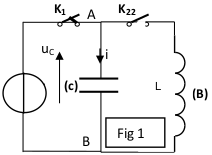
\includegraphics[width=0.25\textwidth]{./ex_011.png}
\end{center}
\end{wrapfigure}


On considère le circuit électrique schématisé dans la figure 4, comportant :

\begin{itemize}
	\item Un générateur de tension continue (G), de f.é.m $U_0$ et de résistance interne \\ négligeable, Un condensateur (c) de capacité C et d’armatures A et B ;
	\item Une bobine (B) d’inductance L et de résistance négligeable ;
	\item Deux interrupteurs $K_1$ et $K_2$.

\end{itemize}




\begin{tabular}{c|l}
	0,5& \makecell[l]{\textbf{1. }$K_2$ étant ouvert, on ferme $K_1$. Après une brève durée, le condensateur porte une charge \\maximale $Q_0$
et emmagasine une énergie électrostatique $E_0$.Donner l’expression de $Q_0$ en fonction\\ de $U_0$ et C.
et l’expression de $E_0$ en fonction de $Q_0$ et C.}\\

\end{tabular}

Le condensateur étant chargé, à t = 0 on ouvre $K_1$ et on ferme $K_2$. A t quelconque, l’armature A du
condensateur porte une charge q.

\begin{tabular}{c|l}
	0,5 & \makecell[l]{\textbf{2. }Exprimer l’énergie électromagnétique E en fonction de L, C, q et $i$.}\\

	0,5 & \makecell[l]{\textbf{3. }Montrer, sans faire aucun calcul que cette énergie se conserve et elle est égale à $\frac{Q_0^2}{2.C}$  }\\

	0,75 & \makecell[l]{\textbf{4. }Déduire l’équation différentielle des oscillations électriques.  }\\
	
	0,5 & \makecell[l]{\textbf{5. }Déterminer l’expression de la période propre $T_0$ en fonction de L et C.  }\\

	1 & \makecell[l]{\textbf{6. }Ecrire l’expression de la charge q en fonction du temps. }\\
	
	0,75 & \makecell[l]{\textbf{7. }Donner l’expression de l’énergie magnétique $E_L$ en fonction de L et i }\\

	1,5 & \makecell[l]{\textbf{8. }Montrer que l’expression de cette énergie $E_L$ en fonction du temps s’écrit :   \\\hspace{3cm}$E_L = \frac{E_0}{2}.\bigg(1+cos\big(\frac{4.\pi}{T_0}.t + \pi \big)\bigg) $ }\\
\end{tabular}

Une étude expérimentale a permis de tracer les courbes (1) et (2) (ci-dessous) traduisant
respectivement les variations de l’énergie magnétique EL en fonction de i et en fonction du temps.

\begin{center}
  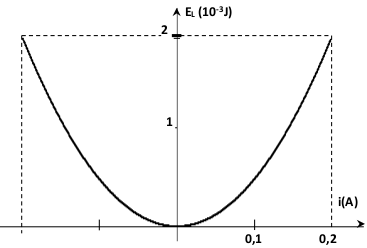
\includegraphics[width=0.5\textwidth]{./ex_01.png}
  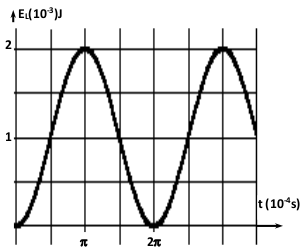
\includegraphics[width=0.43\textwidth]{./ex_02.png}
\end{center}


\begin{tabular}{c|l}
	0,25 & \makecell[l]{\textbf{9. }En exploitant les courbes , Déterminer la valeur de $T_0$. }\\
	1,75 & \makecell[l]{\textbf{10. }déduire la valeur de $C,Q_0$ et $U_0$ }\\


\end{tabular}



\end{document}
